\chapter{Concept Glossary}
\label{app:concepts}

\section{Part I}
\label{app:concepts-p1}
\subsection{Bases, DNA and Variants}

...DNA is made up of four bases; G, C, T and A...


\subsection{Next Generation Sequencing}

...the process of recovering or extracting the sequence of nucleotide bases...


\subsection{Variants and SNPs}
\label{sec:p1-concept:variants}

...for the purpose of this study we are only interested in single nucleotide
polymorphisms (SNPs) "snips" ...

...their \textit{position} refers to the index of the base of the chromosome in
which the polymorphism exists...
...commonly these are 1-indexed (although this is not always the case) and thus
care must be taken to ensure this is accounted for at any step where positions
are considered...

...SNPs...

\textbf{variant calling} - the process of identifying bases in a sample that
differ from the reference genome (this is a little simple as you also need to
discern as whether the difference is actually a polymorphism or not).



\subsection{Samples, Lanes and Lanelets}
\label{chap:samplelanelanelets}
\ifpdf
    \graphicspath{{Chapter2/Figs/Raster/}{Chapter2/Figs/PDF/}{Chapter2/Figs/}}
\else
    \graphicspath{{Chapter2/Figs/Vector/}{Chapter2/Figs/}}
\fi

A \textbf{sample} is a distinct DNA specimen extracted from a particular person.
For the purpose of sequencing, samples are pipetted in to a \textit{flowcell}
such as the one in Figure~\ref{fig:flowcell} -- a glass slide
containing a series of very thin tubules known as \textbf{lanes}.  It is
throughout these lanes that the chemical reactions involved in sequencing take place.

\begin{figure}[htbp!]
    \centering
    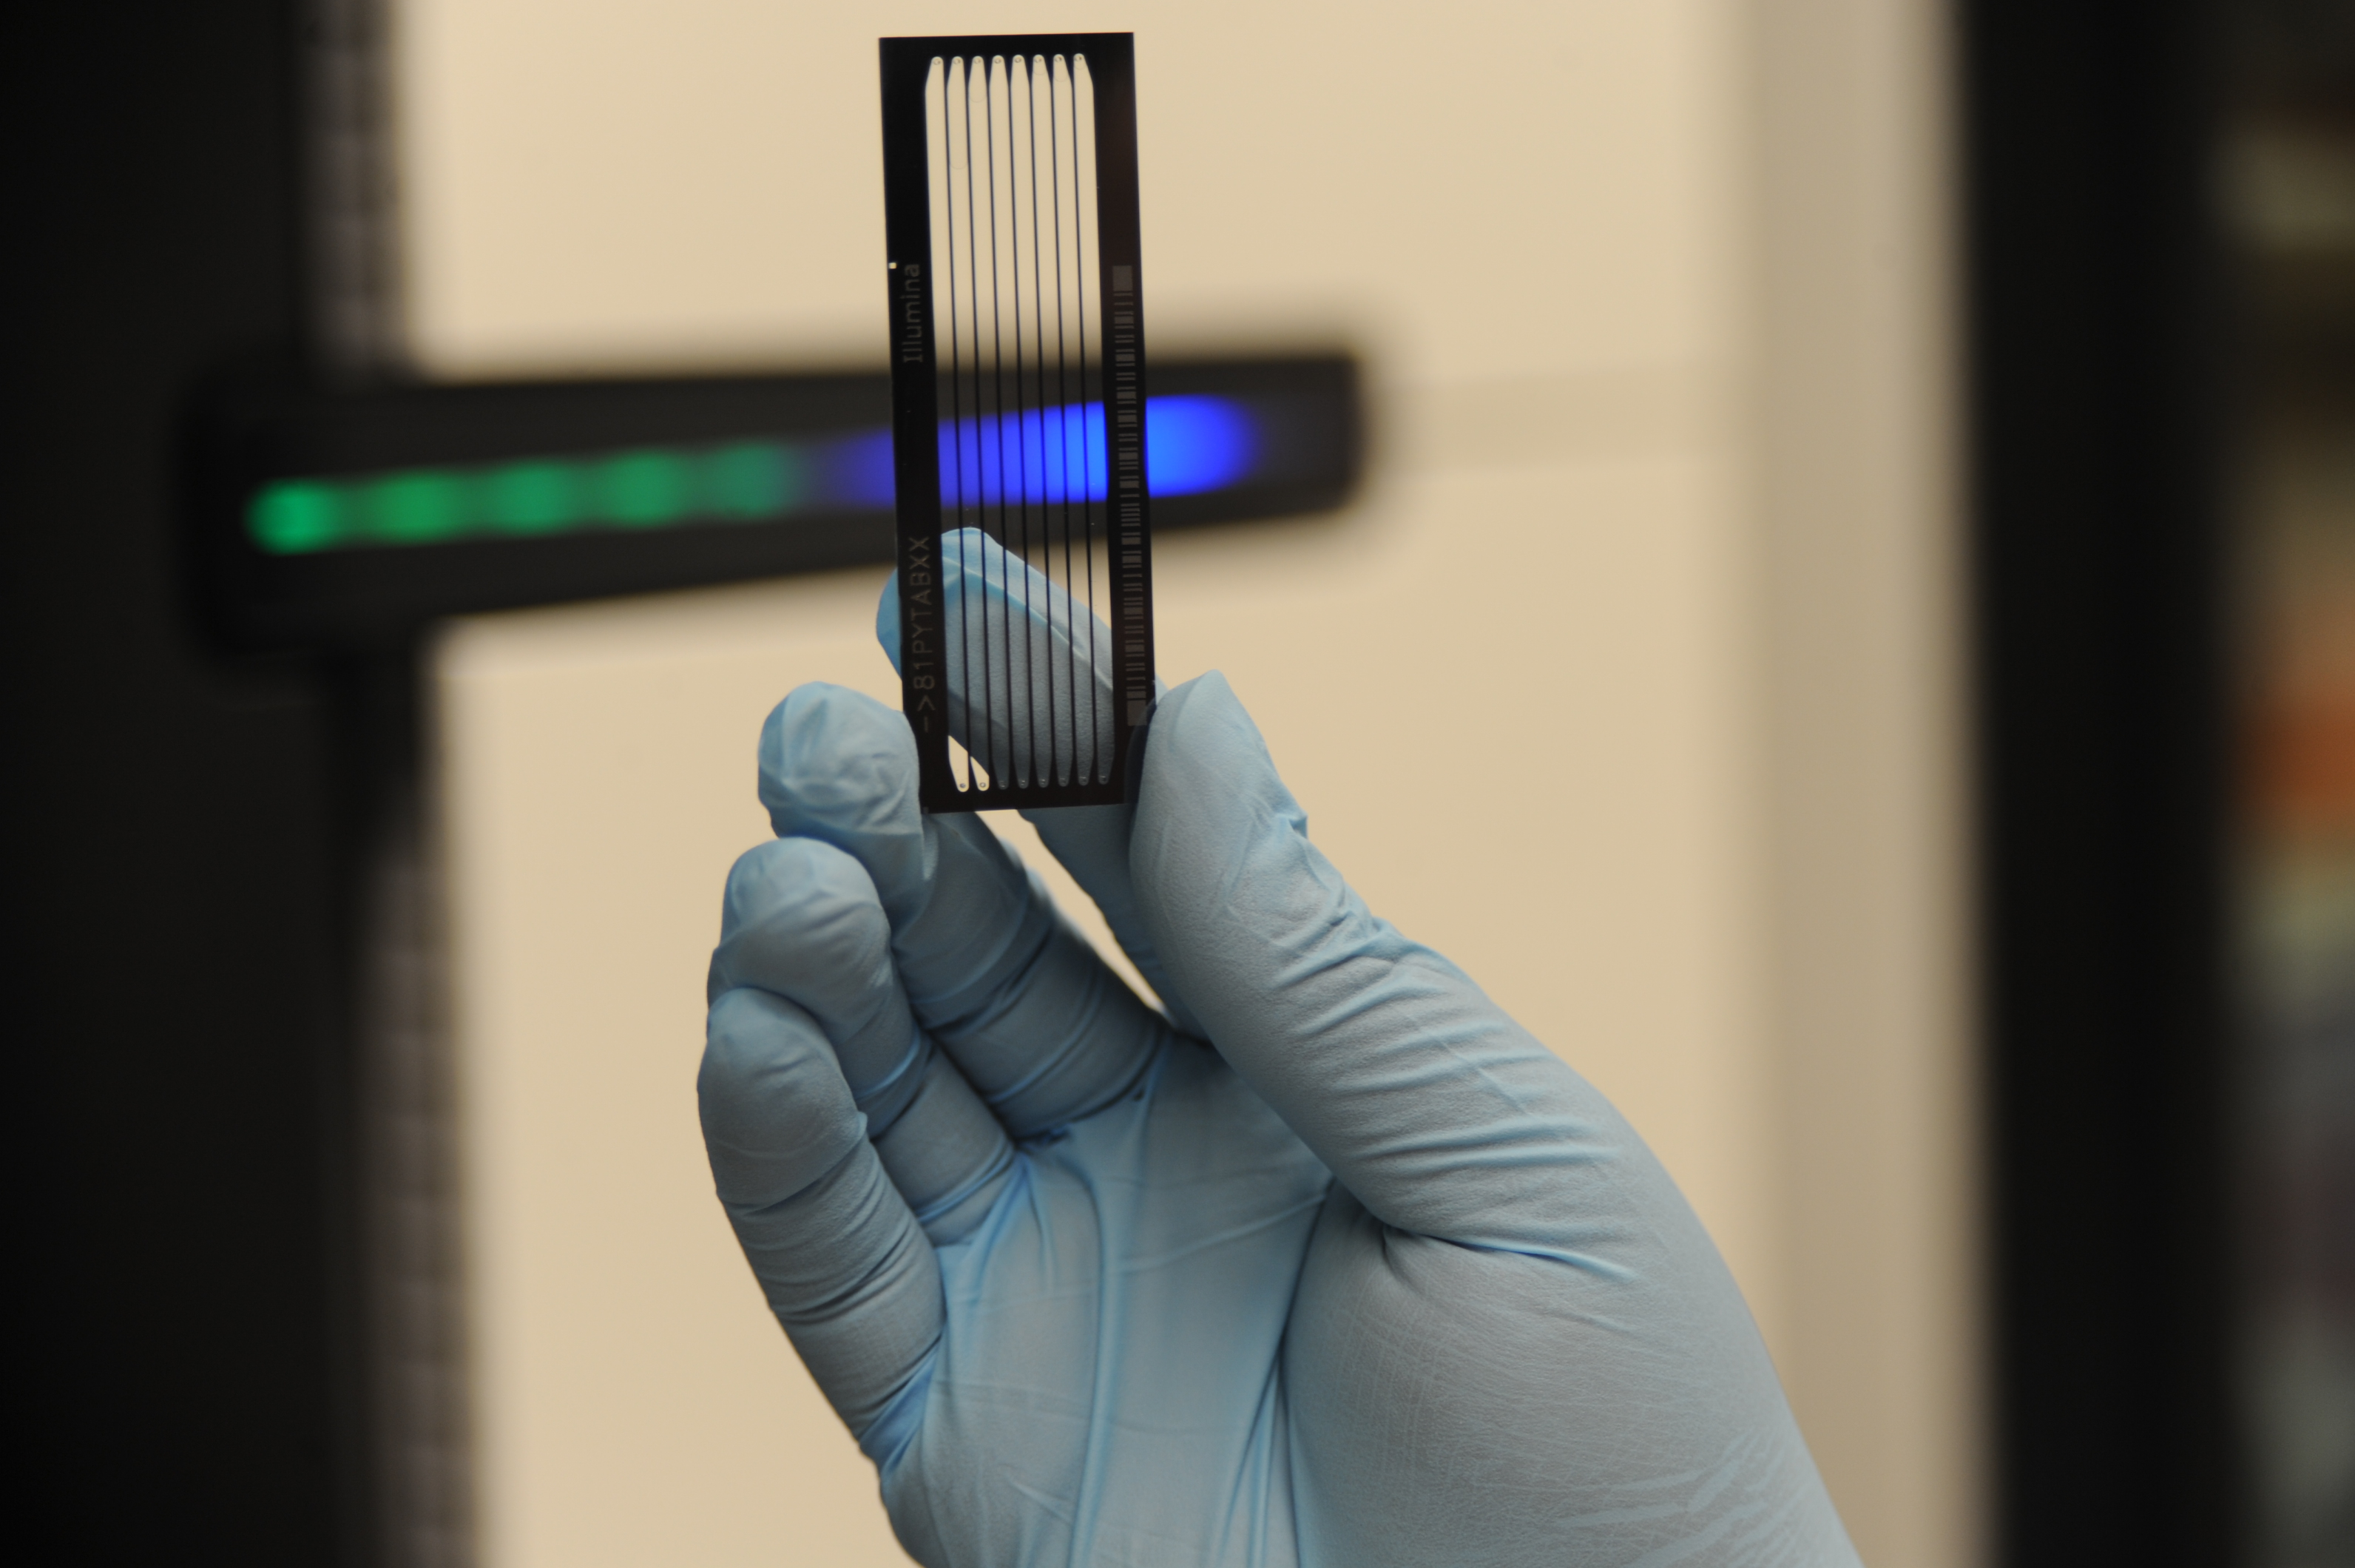
\includegraphics[width=0.4\textwidth]{NHGRI-80102}
    \caption[flowcell]{An Illumina HiSeq Flowcell\citep{img:flowcell}}
    \label{fig:flowcell}
\end{figure}

Once inserted, samples are amplified \textit{in situ}, in the flowcell itself. A
process in which the genetic material of each sample is caused to multiply in
magnitude to form a dense cluster of the sample around the original. Millions of
clusters will be created throughout each lane of the flowcell.

Note that a lane can contain more than one sample and a sample can appear in
more than one lane; this is known as \textit{sample multiplexing} and helps to
ensure that the failure of a particular lane does not hinder analysis of a
sample (as it will still be sequenced as part of another lane).

The more abstract of the definitions, a \textbf{lanelet} is the aggregate read
of all clusters of a particular sample in a single lane.

%Figure~\ref{fig:lanelets} attempts to highlight examples of a this (circled in
%blue -- not all lanelets are highlighted). For example Lane 5 shows the four
%clusters (in reality there would be millions) of Sample A combine to
%represent a lanelet. A lane will have as many lanelets as it does samples.


%TODO Draw a vector of the lanelets diagram
%\begin{figure}[htbp!]
%    \centering
%    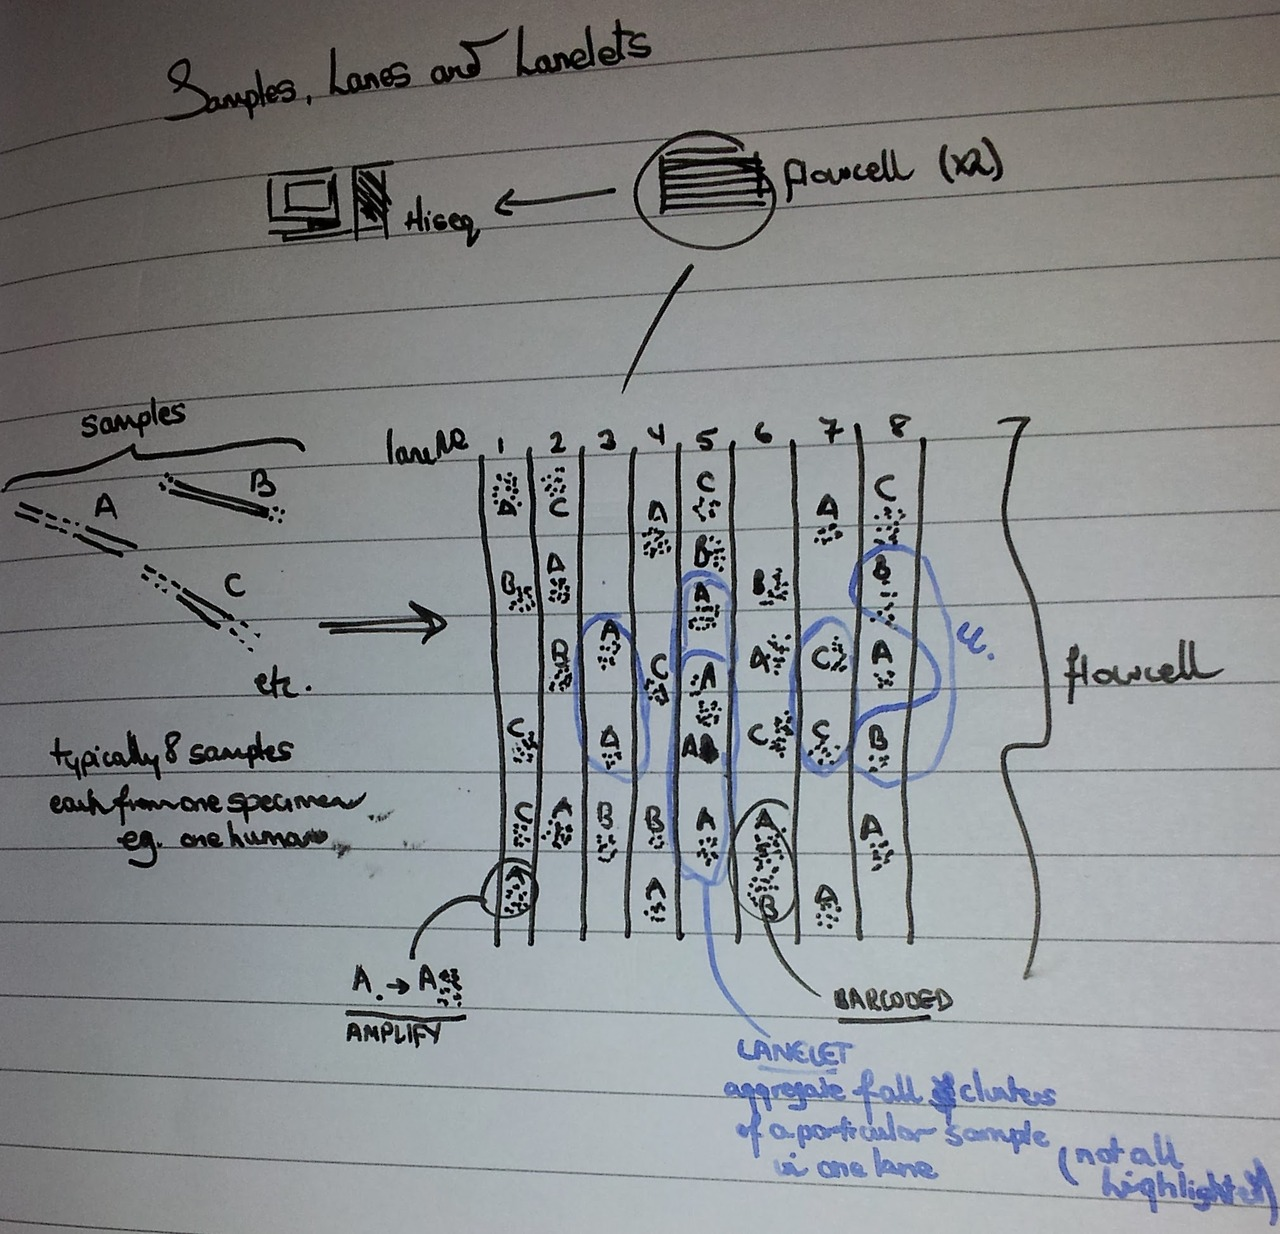
\includegraphics[width=0.5\textwidth]{lanelets}
%    \caption[lanelets]{Example of flowcell with some lanelets highlighted}
%    \label{fig:lanelets}
%\end{figure}

\subsection{Observations and Parameters}

An \textbf{observation} refers to a distinct object or "thing" from which we
will attempt to understand the relationship between its known properties and
classification to be able to label future observations with unknown class based
on those properties. In the context of this project, this would be a lanelet.
Other documentation in the field may use the term \textit{sample} but to avoid
confusion with the definition of sample introduced in
Chapter~\ref{chap:samplelanelanelets} we will use the term observation.

The aforementioned \textit{properties} or \textit{attributes} of an observation
will be referred to as the \textbf{parameters} of that observation.
Traditionally these may be described as \textit{features} but it was felt that
this wording may have connotations with discrete data. Early versions of
Frontier referred to parameters as \textit{regressors}, using terminology from
statistical modelling. This wording was dropped to remove any confusion between
regression and classification machine learning problems.


\subsection{Data and Targets}
%TODO Mention dependent and explanatory variables?

\textbf{Data} will be used somewhat generically to refer to a matrix in which
observations act as rows and their parameters act as columns. It is expected
that all observations will have the same set of parameters.

For problems of a classification nature such as ours, an observation's
\textbf{target} is the known classification of that particular observation.
Depending on the context of the learning problem targets may be discovered
manually (\textit{e.g.} counting leaves from images of plants, one will need to
manually count all the leaves in the image before being able to use it for
learning) or as the output from another system such as \textbf{auto\_qc}.

In the context of this project where the objective is to begin learning the
rules of \textbf{auto\_qc} the targets refer to whether a particular lanelet
observation was labelled as a pass, fail or warn by the current system.


\subsection{Class Labels and Codes}
\label{chap:labelcode}

An observation's target may also be known as its \textbf{label}. A labelled
observation is said to be a member of that label's \textbf{class}. For example a
lanelet that has failed \textbf{auto\_qc} is said to be labelled as a fail and
is a member of the class of failures.

String based class labels can pose difficulties when handling data later on, not
only taking more memory to store as opposed to a type such as an integer but
also introducing accidental subsetting or discarding of data whose labels differ
unexpectedly. For example are "fail", ,"fial", "FAIL" and "Failed" supposed to
be members of the same class?

%TODO Why?
Often such labels are \textbf{encoded} in to simpler types such as integers.


\subsection{Training and Testing}

...

\subsection{Python Data Structures}
\label{sec:python-structures}
%TODO Find better citation (Python book)

The Python standard library offers many different data structures each with
their own properties. I introduce three such structures below to assist the
reader in understanding some of the implementation decisions made in the
following section:

\subsubsection{List}
A \textbf{list}\citep{py-list} essentially represents an ordered sequence of
elements. \textit{Lists} are incredibly versatile, allowing elements of any data
type, including \textit{lists} and other container structures or arbitrary
objects. Elements in a \textit{list} are accessed by their index (location)
in the sequence. \textit{Lists} permit duplicate values.

\textit{Lists} are represented in memory as a contiguous block and so great
expense is incurred if the \textit{list} grows beyond its bounds and must be
relocated elsewhere in memory to resize to a larger contiguous block.
Whilst items can be appended to or popped from anywhere in the container,
performing those actions on a location that is not at the end of the
\textit{list} will require the contents of the structure to be moved in memory
to maintain the contiguous layout.

%TODO Cite time
Checking whether an item is in a \textit{list} requires iterating over all $n$
elements in the container until either a match is found or there are no elements
left to check.


\subsubsection{Dictionary}

A \textbf{dict}\citep{py-dict} or \textit{dictionary} is a structure containing
key-value pairs in which string or numeric keys\footnote{Any type can actually
be used as a dictionary key providing it is immutable, including
tuples\citep{py-dict}} are mapped to an arbitrary value or object through a
hashing function. Keys in a \textit{dictionary} are unique; attempting to add a
key-value pair where the key already exists will overwrite the original entry.

%TODO Cite time
Python \textit{dictionaries} offer constant lookup access and more importantly,
unlike a list, querying the structure for whether it contains a particular key
can be performed in constant time\citep{py:timecomplexity}.
However it is important to note that a \textit{dictionary} does not maintain
order, keys are not sorted alphanumerically nor are they sorted by insertion
time. Ordering is determined arbitrarily by the \textbf{dict}'s underlying hash
table\footnote{This is probably the question I see most often from users new to
Python on StackOverflow}.


\subsubsection{Set}

\textbf{Sets}\citep{py-set} represent a collection of elements and are similar
to a \textbf{dict} in that they are allowed to contain any immutable (thus
hashable) elements but entries are not mapped to a value or object.
\textit{Sets} are forbidden from containing duplicate objects and do not
maintain order.

%TODO Cite time
Like \textbf{dict}, checking for membership of an item in a \textit{set}
completes in constant time, making the structure particularly useful for
membership testing and filtering duplicates out of other structures.



\section{Part II: Goldilocks}
\label{app:concepts-p2-1}
\subsection{Group}
%TODO Reads a bit poorly

Rather than considering the location of all variants in our samples as a whole,
we may wish to consider how variants are distributed across the two different
data sets we have, namely the \textbf{GWAS} and \textbf{iCHIP} sets. Thus variants
will be considered as members of a \textbf{group}. The group may be
arbitrarily defined but for the purpose of our own analysis the set in which a
variant appears will be considered as its group.

A particular variant location may appear in more than one group.


\subsection{Length and Stride}
\label{sec:lengthstride}

The \textbf{length} of a region represents the number of bases included in the
region and the \textbf{stride} refers to the number of bases to be used as an
offset between the first base of one region and the beginning of the next.

Sensible choices for these parameters will need to be selected after considering
both time and memory.


\subsection{Density}

The \textbf{density} of a region represents the number of variants located
within that region. \textbf{Density} will be recorded for each \textit{group} of
variants.


\subsection{Candidate Regions}

A \textbf{candidate} is a region of \textit{length} bases whose first base falls
on a \textit{stride}. A \textbf{candidate} region will contain some count
(described as the \textit{density}) of variants for each group. In the context
of this project we consider the number of variant locations that fall within
this region for both the \textbf{GWAS} and \textbf{iCHIP} data sets.

\textbf{Candidates} must meet all (any any additional) criteria to be considered.
For example, regions whose first position falls on a base in such a way that the
chromosome ends before a region of \textit{length} can be constructed will
violate the size criteria.

\section{Part II: Pipeline}
\label{app:concepts-p2-2}
%TODO Concepts: Genotype Likelihood?

\subsection{htslib}
...high-throughput sequencing library...

\subsection{samtools}
\subsection{bcftools}
...spun off from the \textbf{samtools} repository...
...now using \textbf{htslib}...

\subsection{SAM and BAM Files}

\subsection{"The Farm"}
%TODO Cite LSF

...Sanger Institute cluster...
..."the farm"...
...jobs submitted and managed through \textbf{LSF}

%TODO Cite internal slides: Introduction to LSF at Sanger
% Farm Users Intro: Informatics System Group
\begin{listing}[H]
    \caption[lsf-memory]{\textbf{LSF Resource Syntax}: \textbf{bsub} flags
        required to raise memory allocation for a job.}
    \label{list:lsf-memory}
    \begin{minted}[%mathescape,
                %linenos,
                gobble=8,
                frame=lines,
                framesep=2mm]{bash}
        bsub -R"select[mem>4000] rusage[mem=4000]" -M4000 ...
        #                 |                |        | Raise maximum job memory to 4000mb
        #                 |                | Pre-reserve 4000mb for job before execution
        #                 | Only run on a node with more than 4000mb memory
    \end{minted}
\end{listing}

\subsection{GWAS Data Set}
...the \textbf{GWAS} is made up two studies...
...one of which used 2x, the other 4x
...due to time constraints we had to discard the smaller 4x study...

